\chapter{Android Forensics}
\label{ch:forensics}
It is impossible to develop techniques for preventing the acquisition of data without understanding how that data would be acquired.
This chapter aims to lay bare the fundamentals of Android forensic acquisition and analysis on the Android 2.3 platform, also called
Gingerbread. Gingerbread is the latest version of Android for which established forensic techniques have been developed.  The
``Technical Background'' section discusses the details of the \texttt{YAFFS2} filesystem, which is used on most Gingerbread devices.
The same section also introduces methods for extracting data from a \texttt{YAFFS2} image.  The ``Acquisition" section focuses on
building and using the tools necessary to acquire a forensically sound image of an Android partition.  Finally, how data can be
pulled from an acquired Android image is described.


\section{Technical Background}

The data presented here has been gathered from a Nexus One phone running Android version 2.3 (Gingerbread).  ``Nexus''
devices\footnote{Nexus One, Nexus S, and now Galaxy Nexus} are often favored by developers, as they provide a build of Android that
is as close as possible to the Android Open Source Project, hereafter referred to as AOSP. While Android is considered by many to be
an open mobile platform, not everything in Android is open-source. AOSP is that part of Android for which the source code has been
released.  It includes the majority of features in a consumer build of Android, but notably excludes many of the Google branded
applications, such as Gmail and the Android Market. Traditionally, AOSP has also excluded proprietary hardware drivers, but recently
many drivers for Nexus devices have been made available.  The consumer builds for Nexus devices are not based on AOSP, but they
are much closer to AOSP than the builds shipped with other models, which often come loaded with third-party applications and
modifications to the underlying operating system.

Before diving into the details of Android forensics, it is important to give a short overview of how Android storage is laid out.
The majority of Android devices have two storage devices: an SD card \footnote{Often an actual, removable SD card is provided with
the phone. Newer devices, however, appear to be trending toward providing an emulated SD card from internal storage.} that is
formatted with a FAT filesystem, and an internal NAND flash that is formatted \texttt{YAFFS2} or \texttt{ext4}, with newer models
preferring \texttt{ext4}.\footnote{There are notable exceptions, such as the Samsung Galaxy S, which uses a proprietary filesystem called RFS.} The SD
card provides a wealth of forensic artifacts, as it is typically on the SD card where large media files such as pictures and music
are stored.  Applications can choose to make use of the SD card for their internal data storage, as well.  Despite its importance,
this paper will not discuss FAT forensics, as it has been discussed at great length elsewhere \cite{carrier}. 

Depending on the particular device, Android 2.3 has up to six partitions, excluding external storage: \texttt{boot}, \texttt{system}, \texttt{cache}, \texttt{userdata},
\texttt{recovery} and \texttt{misc}. 
The \texttt{boot} partition houses the kernel and a ramdisk.
The \texttt{system} partition holds all of the operating system files, including any of the core applications that are distributed with Android, such as the browser. 
The \texttt{cache} partition provides a scratch space for temporary files, such market downloads.
The \texttt{userdata} partition is where the vast majority of application data is stored.
The \texttt{recovery} partition is used to flash updates and new versions of Android on to the phone. 
The \texttt{misc} partition is used to store miscellaneous hardware settings.
Undoubtedly, from a forensic perspective, the \texttt{userdata} partition is the most interesting, and what will be focused on in
this paper. The other partitions do hold valuable information, but at a much lower density.
\footnote{Even though this paper does not discuss partitions outside of \texttt{userdata}, from a privacy perspective it is
important to realize that sensitive information could still be leaked by other partitions, particularly \texttt{cache} and the SD
card.}

To determine the partition layout of an Android device:

\paragraph {1. 
Enable USB Debugging} Figure \ref{fig:usbdebug} shows the \texttt{Development} menu for Android 2.3, where USB Debugging can be
enabled.  Turning on USB debugging allows shell access to the device without entering a passcode. The shell is accessed with a
utility called the ``Android Debug Bridge,'' or ADB. Enabling USB debugging does not provide root access to the device, but it is
often easier to execute a privilege escalation attack from within a shell than from the Android interface. Any passcode that is
enabled must be first bypassed before USB debugging can be enabled, unless debugging was previously enabled by the device owner.
There are a variety of techniques for bypassing a passcode \cite{hoog, lockscreenbypass0, lockscreenbypass1, lockscreenbypass2}, but
there is no single method that is consistently successful across devices.  A strong passcode remains a significant barrier to
accessing the information on a device.

\begin{figure}[ht]
\caption{Turning on USB Debugging}
\begin{center}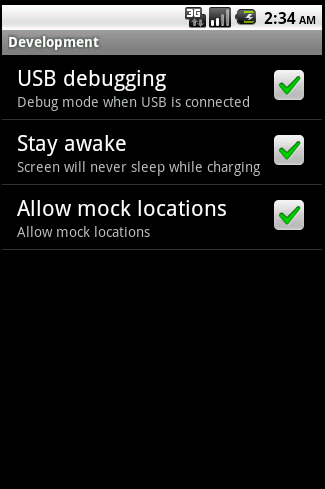
\includegraphics[scale=0.5]{usbdebug.png}\end{center}
\label{fig:usbdebug}
\end{figure}

\paragraph {2. Open an \texttt{adb}  Shell}

The Android Debug Bridge (\texttt{adb}) is the primary means by which a developer or forensic analyst will communicate with an
Android device. It is provided as part of the Android Software Development Kit (SDK), or can be built as part of the process of
building the AOSP platform. The SDK provides an \texttt{adb} binary in \texttt{\$SDKPATH/platform-tools}, and the build process puts
\texttt{adb} in \texttt{\$BUILDROOT/out/host/linux-x86/bin}.\footnote{Google has provided excellent instructions at
\texttt{source.android.com} for building AOSP from source code.}  The Android Debug Bridge is the only practical way to obtain
low-level access to an Android device without physically removing the NAND chip.

When \texttt{adb} is first run, it starts a service that is then used to connect to the Android device. 
Once the \texttt{adb} service is started, a list of attached Android devices can be shown using the command \texttt{adb devices}. 
The output of \texttt{adb devices} from a machine with one Android phone attached is shown in Figure \ref{fig:adbdevices}.

\begin{figure}[ht]
\caption{ADB Connected Devices}
\begin{center}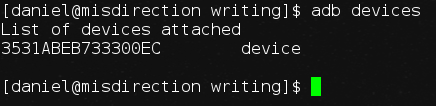
\includegraphics[scale=0.6]{adbdevices.png}\end{center}
\label{fig:adbdevices}
\end{figure}

Opening a shell and displaying the contents of \texttt{/proc/mtd} results in output similar to figure \ref{fig:mtd}.  MTD is the
kernel driver in Linux that is responsible for providing the abstraction layer that is between filesystems and \emph{Memory
Technology Devices}, i.e. NAND flash. YAFFS2 is a consumer of the MTD interface, and \texttt{/proc/mtd} lists all of the active MTD
partitions. 

\begin{figure}[ht]
\caption{MTD Partition Layout of an Android Phone}
\begin{center}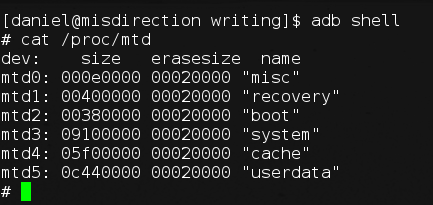
\includegraphics[scale=0.6]{procmtd.png}\end{center}
\label{fig:mtd}
\end{figure}	

This layout was taken from a Nexus One running Gingerbread.  All of the information in \texttt{/proc/mtd} is valuable and should be
recorded when seizing a mobile device. The first column is the device name which corresponds to the device handle in
\texttt{/dev/mtd}.  The second column shows the size of each partition in bytes. 
The third column gives the ``eraseblock'' size for the partition.  Eraseblocks are the MTD equivalent of sectors in a conventional block
device \cite{mtdfaq}. The eraseblock size determines what the smallest chunk of data is that can be accessed on an MTD.  When an MTD
is presented as a virtual block device, so that it can be mounted by a filesystem, the eraseblock size becomes the block size.  Each
block will consist of many NAND pages, which are the smallest unit of data that the NAND device itself supports.  NAND pages are
typically 2048 bytes, but the exact page size can be determined by looking at \texttt{dmesg} shortly after the phone boots.  The
fourth and final column in \texttt{/proc/mtd} shows the friendly name of each partition.  The output of a standard \texttt{df}
command will show where each device is mounted.

\subsection{YAFFS2 - Yet Another Flash File System}
Most Android devices still use YAFFS2 as the filesystem of choice for user data that is not stored on an external SD card.  YAFFS2 is
very different from other filesystems such as NTFS or FAT32.  YAFFS was the first filesystem specifically designed for NAND flash,
and so its structure is optimized for the specific requirements that NAND flash imposes.  Chief among these is the limit on the
number of overwrites performed.  NAND pages have a finite lifetime, and a filesystem that does not distribute wear will quickly wear
out some pages.  The pages storing the FAT in FAT32, for example, would quickly become corrupt without a hardware flash translation
layer (FTL), as is used in thumb drives.  YAFFS2 is designed to operate without a hardware FTL, which is good news for forensic
investigators, as it affords a software view into the flash device.  Overwriting NAND pages requires that those pages first be
erased, which in NAND incurs a heavy performance hit.  This leads to what is known as the ``write once" requirement, which is that
NAND pages should only be written to once until it is absolutely necessary to overwrite them. The write once requirement has
influenced the design of YAFFS2 more than any other single factor.

YAFFS2 is known as a ``log-structured'' filesystem.  A log-structured filesystem does not reuse flash pages when a piece of data is
updated.  Rather, it simply writes the updated data to the next available location.  A monotonically increasing sequence number
keeps track of which data is most current, and the older versions of the same data are ignored.  This has dramatic forensic
implications, as it often means there are hundreds of copies of a given piece of data, even after it has been deleted.  YAFFS2 does
have a garbage collection routine that periodically erases old chunks in the background, but this routine appears to run
infrequently enough that forensic analysis of deleted data in YAFFS2 is still a valuable source of evidence \cite{naval}. 

Before we can understand how YAFFS2 stores data, we need to look at its predecessor, YAFFS1.\footnote{The filesystem was actually
just called YAFFS, but for the sake of clarity it is here referred to as YAFFS1.} Every piece of data written to a YAFFS1 based file
system is written in the form of a ``chunk", which is always the same size.  There are data chunks which hold the actual data in a
file, and there are object header chunks, which hold metadata about objects such as directories, files, and the like.  Each chunk in
YAFFS1 has the following information associated with it:

\begin{itemize}
	\item {\bf ObjectId}: Identifies which object the chunk belongs to.\
	\item {\bf ChunkId}: Identifies where in the file this chunk belongs. 
		A chunkId of zero signifies that this chunk contains an object header. 
		ChunkId 1 is the first chunk, ChunkId 2 the second, and so on.
	\item {\bf Deletion Marker}: Shows that this chunk is no longer in use.
	\item {\bf Byte count}: Number of bytes of data if this is a data chunk.
\end{itemize}
\cite{howyaffsworks}

YAFFS1 relies on the Linux kernel's Memory Technology Device (MTD) driver to provide an interface to the actual NAND device.  The
Linux MTD presents the NAND device as a series of pages (usually 2kB), similar to blocks on a conventional hard disk.  Each page is
accompanied by 64 bytes known as the ``Out-of-Band area," or OOB, which is partially used by the MTD itself and partially used by
the YAFFS1 filesystem. The MTD driver itself uses the OOB area to store error correction data, and additionally defines an area that
can be used by the filesystem for whatever purposes it chooses, called the OOBFREE area.  The layout of the OOB can be seen in the
\texttt{struct} in Table \ref{tab:oob}, taken from the Android source code. This \texttt{struct} is extremely important for anyone
attempting to analyze a YAFFS based filesystem.

\begin{table}
\lstinputlisting{tables/oobstruct.c}
\caption{Out-of-Band Area (OOB) \texttt{struct}}
\label{tab:oob}
\end{table}

The most important part of this struct, for our purposes, is the definition of the \texttt{oobfree} array.  The first element of the
\texttt{oobfree} array gives the offset into the area that is available for filesystem usage, and the second element determines the
size of that area.  There may be multiple arrays in \texttt{oobfree} leading to complex, non-contiguous free areas, but Android
appears to use one contiguous block.  This is not the standard layout used by Linux. Every file and directory within a YAFFS based
filesystem has an object header that is stored with this OOBFREE area. The object header describes the contents of the object, which
is stored in the data area of the chunk. This object header will include the object name, type, and length.  Notice that because the
object header contains the length, it must be written to every time the file length is changed.  Because YAFFS writes sequentially,
the new object header will be placed at the end of the object (with the same chunk id), and the old object header will be marked
deleted. 

YAFFS1 and YAFFS2 are actually remarkably simple compared to other file systems. To reiterate, the NAND device is divided into
pages, each with a small area for metadata (OOB).  The OOB defines what type of chunk that page belongs to, which chunk the page
belongs to, and in turn which object that chunk belongs to.  In YAFFS1 it also marks whether or not that chunk has been deleted.
Each object has a single object header and zero or more data chunks.  That's it.  Notice the conspicuous lack of any central
metadata location.  This makes the filesystem exceedingly simple, but at the price of \emph{scanning the OOB area of every page at
boot}.  There is no actual filesystem structure maintained on disk, just object headers and data chunks.  The filesystem layout is
determined at scan time and maintained in memory only. 

YAFFS2 is only slightly different than YAFFS1. The biggest change was the removal of the deletion marker, which was replaced with a
sequence number. Each time a page is written to it increases the sequence number by one, allowing pages with the same chunk id and
the same object id to be differentiated.  Whichever page has the largest sequence number is used, and the others are ignored.  Also,
in YAFFS2 the concept of a checkpoint was introduced, which essentially stores a snapshot of the data structures maintained in
memory, allowing for a faster boot.

\subsection{Carving SQLite Records Out Of YAFFS2}
A large percentage of forensically interesting information on an Android phone is indexed in SQLite databases.  The majority of
these databases are stored on the \texttt{userdata} partition of the phone, mounted at \texttt{/data}.  Pulling data from these
SQLite databases while they are intact is trivial.  Simply open the relevant database with SQLite and query the data.  It becomes
more interesting when the data has been overwritten or deleted.  Murilo Tito Pereira has done excellent work on carving for deleted
SQLite records, and his article on carving Firefox SQLite databases forms the basis for the forensic methods presented this section.
\cite{carvefirefox}

The database used by the Android browser is a good example. The browser actually has several databases, but for now
\texttt{browser.db} will suffice. The browser database is stored at \texttt{/data/data/com.android.browser/databases/browser.db},
and contains three tables: \texttt{android\_metadata}, \texttt{bookmarks}, and \texttt{searches}.  The bookmarks table contains
entries for not only bookmarks but browser history as well.  The searches table contains search history. 

\begin{table}
\begin {center}
	\begin{tabular}{| c | c | c |}
	\hline
	Field & Type & Comment \\
	\hline
	\_id & INTEGER PRIMARY KEY & \\
	title & TEXT  &  Only used for bookmarks \\
	url & TEXT  & Location of bookmark or history visit \\
	visits & INTEGER  & Number of times site has been visited \\
	date & LONG  &  Last visit \\
	created & LONG &  Date created \\
	description & TEXT &  User entered description \\
	bookmark & INTEGER & Whether or not record is bookmark \\
	favicon & BLOB &  For webpages \\
	thumbnail & BLOB &  Shown in bookmarks screen \\
	touch\_icon & BLOB &  Unknown \\
	user\_entered & BLOB & Boolean, created by default or not \\
	\hline
	\end{tabular}
\end{center}
	\caption{Bookmarks Table Schema}
	\label{tab:bookmarkschema}
\end{table}

Knowing the table schema of the records being searched for is of the utmost importance.  If all an investigator is interested in is
seeing what was in a database when the phone was acquired, then the database file can be extracted from the image and opened in
SQLite explorer.  If, on the other hand, the investigator is interested in records that may have been deleted, then the filesystem
must be carved for structures that match the table schema.

Following Pereira's work on carving for deleted Firefox history records, an Android image can be scanned for unallocated SQLite
records.  Updating a record in a SQLite database stored on a YAFFS2 filesystem does not immediately overwrite the old record
(remember YAFFS makes every effort to write sequentially).  From a forensics perspective, it is interesting to note that using the
native Android tools to clear browser history does not remove the filesystem artifacts left by YAFFS2 wear-leveling mechanisms.
Eventually the artifacts will be erased by the filesystem garbage collector, but on a phone with a significant amount of free space,
that can take a very long time.

The approach taken by Pereira, which has here been adapted and somewhat generalized, is to search for a signature that is unique to
the content of the deleted record one is attempting to locate.  Pereira was looking for Firefox browsing history records in
unallocated space, so he used \emph{http://} for his signature.  When looking for browsing history records on an Android based
phone, the same signature can be successfully used.  The signature chosen depends on the records one is looking for.  One might use
the regular expression \verb|\d{3}-\d{3}-\d{4}| to search for SMS records floating around the filesystem, as those records are guaranteed
to have a phone number field (the actual field name is \texttt{address}). 

Clearly a signature alone, however, is insufficient to distinguish SQLite records from other occurrences of the signature.  The
signature is only used to locate candidate records, which then must be validated.  This validation is accomplished by stepping
backward from the signature location, counting bytes.  The first value after the \texttt{id} in a SQLite record is the header size.
If the number of bytes that have been stepped over, minus the number of bytes in data fields based on the record schema, is equal to
the value of the byte the cursor has landed on (the header size), then a potentially valid SQLite record has been located.  The fact
that the byte after the header size must by definition be zero is used as a sanity check.

This project implemented SQLite validation in Python, using two functions.  One function ``backsteps'' from a given signature
passing progressively larger slices to a validation function.  The validation function returns whether or not the slice could be a
SQLite record.  The \texttt{backStep} function is shown in table \ref{tab:backstep}. 

\begin{table}
\lstinputlisting{tables/backstep.py}
\caption{SQLite Carving Backstep Function}
\label{tab:backstep}
\end{table}

The \texttt{rawData} argument passed to \texttt{backStep} is simply a slice of data that is larger than the record is believed to
be.  When searching for browser history records, for example, this project opted for 512 bytes on either size of the record.  The
size is arbitrary, so long as it is larger than the record being searched for, but choosing a raw data slice size that is too large
will negatively impact validation performance.  The \texttt{bc} variable (backward cursor) is the current byte location.  The
function starts by initializing a zero list that equals the size of the record (data only) as determined by the expected schema for
that record type.  The function then proceeds to step backward one byte at a time, calling \texttt{validateHdr} with a slice of raw
data.  If the current slice appears to be valid, then all of the data after the signature is stored in \texttt{tailingRec}, and
\texttt{validateHdr} will have already have populated the header data.  The \texttt{validateHdr} function does the comparison
between the record schema and the header and field sizes that have actually been found.  Effectively, the function does brute force
carving by taking incrementally larger slices of data and testing for validity against the table schema.

\section{Acquisition}
At this point, the structure of the filesystem on an Android 2.3 device has been covered, as well as an example of carving
forensically useful data from the device. But how was this data retrieved in the first place? In a digital investigation, the
primary source of evidence is a copy of the target device's nonvolatile data.  Acquiring the nonvolatile data, be it from a
conventional hard disk or from NAND flash in a mobile device, is known as ``post-mortmem'' acquisition, because the data is
collected after the device has been powered off.  Post-mortem acquisition is a well-established process, standing in contrast to
live system acquisition, which is a relatively new and quickly evolving process, even for desktop and laptop computers.  Forensic
acquisition of mobile devices follows the same principles as more traditional forensic acquisitions, but the tools, techniques, and
limitations can be very different. The process of acquiring a system, whether it be a desktop or a mobile device, is of primary
interest to digital investigators and incident responders. They typically adhere to procedures and practices that create
``forensically-sound'' duplicates.  According to Craig Ball, 

\begin{quote}
“A ‘forensically-sound’ duplicate of a drive is, first and foremost, one created by a method which does not, in any way, alter any data on the drive being duplicated. 
Second, a forensically-sound duplicate must contain a copy of every bit, byte and sector of the source drive, including unallocated ‘empty’ space and slack space, precisely as such data appears on the source drive relative to the other data on the drive. 

\hspace{\fill}\cite{ball}
\end{quote}

The forensically-sound duplicate outlined by Ball is usually acquired by physically removing the hard disk from the target system.
The hard disk is then attached to a write blocking device and copied using one of many possible acquisition utilities, creating an
``image" of the drive. For analysts of average means, creating a forensically-sound duplicate of an Android device can be
challenging. The operating system itself and the majority of forensic artifacts (with the exception of pictures, media files, and
some application data) are stored on internal flash memory.  Removing the flash memory and attaching it to a write blocker is, while
technically possible, beyond the reach of many forensic labs.  The NAND memory in many devices could conceivably be accessed either
through the JTAG\footnote{JTAG stands for ``Joint Test Action Group.'' JTAG test access ports are available on most circuit boards.
They are used to access the CPU to perform debugging operations, and in certain situations can be used to bypass security mechanisms
or directly access NAND storage.} ports in the device, or by physically removing the chip.  Either method would require significant
electronics work and further reconstruction of the low-level NAND layout. Directly accessing the NAND flash is a last resort, but it
may be the only possibility on a properly locked device \cite{chipoff}.

Further challenges are presented by the inability of standard users to perform the low-level operations necessary to forensically
acquire a device, as the Android security model does not usually provide root access.  Additionally, flash memory stores metadata in
a fashion that is not taken into account by traditional forensic acquisition methods.  The sections that follow describe the
peculiarities of Android and how to approximate a forensically-sound duplicate of an Android device.

\subsection{A Basic Android Acquisition}

The acquisition of an Android device is not, in a broad view, much different than the acquisition of a desktop computer. 
The device must be seized, and an image of the device must be created that is as forensically sound as possible.  There are,
however, several Android specific details that must be addressed.  What follows is an overview of the steps necessary for acquiring
and Android device, partially drawn from Andrew Hoog's book \emph{Android Forensics} \cite{hoog}.

% Vboxes prevent page breaks between item descriptions and item text
\begin{description}
\vbox{\item[Step Zero] Build tools and Document Procedures \hfill \\
Perhaps it goes without saying, but it is imperative that the acquisition tools and procedures be developed \emph{prior} to acquisition. 
If the phone is using YAFFS2 as the filesystem (the majority of devices at the time of writing), \texttt{nanddump} should  be used. 
The process of building \texttt{nanddump} from source is described later in the chapter. 
The Android Debug Bridge, provided with the Android SDK as a means of communicating with the phone over a USB cable, should be installed and tested. }

\vbox{\item[Step One] Initial Seizure \hfill \\
Regardless of the method used to acquire the phone, it must first be secured in the analyst's possession, physically and
electronically.  If the phone is unlocked, immediately determine if a passcode is enabled.  Determine, to the best of the analyst's
ability if the phone is using full disk encryption; if so, do not turn off the phone.  If the phone is encrypted and already off,
then more creative methods will need to be employed (see chapter \ref{ch:fde}).  The version of Android should be retrieved from the
settings menu prior to shutting the phone down.  USB should be enabled if possible.  Unless a logical analysis is going to be
performed, or the phone is encrypted, it should be powered off.  Isolate the phone from the network, either by turning it off or
placing it in a Faraday bag.}

\vbox{\item[Step Two] Back at the Lab \hfill \\
If the device is locked, the password will need to be guessed or bypassed, either through brute-force or a smudge attack.  A smudge
attack involves reading the residual oil patterns off of a touch screen in order to determine the unlock pattern or PIN
\cite{smudge}. The SIM card should be removed and analyzed separately, though SIM cards used in Android devices do not make
particularly interesting pieces of evidence as the majority of data is stored on the phone itself.  If removable, the SD card should
also be removed and analyzed separately (in the same fashion as a thumb drive). A sterile (zeroed) SD card should be placed in the
device for storing NAND images. 
}
 
\vbox{\item[Step Three] Root the phone \hfill \\
If the phone does not already have root access enabled, then privilege escalation will be necessary.  A substantial amount of
research should be done about every device before attempting to obtain root access.  There is a considerable amount of risk of
damage to the phone, including loss of evidence.  Some phones can be rooted with a minimal footprint, as described later in this
chapter.  Other's phones require more invasive processes.  Any analyst of modest means (i.e. without an exploit development team) is
at the mercy of the security/hobbyist community for root access.}

\vbox{\item[Step Four] Acquire an image \hfill \\
Use \texttt{nanddump} to acquire an image of each partition of the phone.  These images should be stored on the sterile SD card that
was inserted into the phone.  After transferring the images from the SD card to the analyst's machine, they can be carved and
mounted with \texttt{nandsim} for perusal.} 
\end{description}

Acquiring an image of an Android phone's filesystem presents a distinct challenge.  The conventional methods of forensic acquisition
are either inadequate or not available.  One of the most popular tools for acquiring an image of a conventional (spinning disk) hard
drive is \texttt{dd}, which reads raw data, block by block, from a one location and writes it to another, which, when the disk is
offline, is sufficient to acquire a forensically valid image of the device.  Unfortunately, \texttt{dd} is not sufficient for the
YAFFS devices, as it operates above the MTD layer. Android images that are acquired by a utility that is not flash-aware have no
hope of being forensically-sound. Such utilities ignore the OOB area of the flash device. YAFFS2 relies significantly on
this OOB free area, and it is therefore of paramount importance that a flash-aware utility is used to acquire any Android image.
Without the OOB area it is impossible to fully reconstruct the YAFFS2 filesystem of an Android device.

\subsection{Nanddump}
Hoog's book \cite{hoog} provides an excellent primer on how Android forensics is performed.  Unfortunately, a great number of
implementation details are glossed over in favor of describing opaque forensic tools, such as Hoog's own AFLogical/AFPhysical tools,
or Cellebrite's more well-known UFED. These tools are only available to the law enforcement community, limiting their academic
value. The tool used here for acquiring Android images is \texttt{nanddump}. The same tool is included in Hoog's tool set, but his
description of cross-compiling \texttt{nanddump} for ARM is limited to: 
\begin{quote} Cross-compiling source code to run on the ARM platform can be quite difficult and there is sparse support for it
online.  One possible solution is to use Android's Native Development Kit (NDK) to build compatible binaries.  Another option is to
use Linux and install a cross-compiler such as Code Sourcery's G++ Lite 2009q3-67 for ARM GNU/Linux from
http:///www.codesourcery.com/sgpp/lite/arm/portal/release1039.  Once a cross-compiler is installed, you must modify the source
code's Makefile to indicate the cross-compiling option.  Also check the book's web site at
http://viaforensics.com/education/android-forensics-mobile-security-book/ for future updates.  \hspace{\fill}\cite{hoog} \end{quote}
The above characterization is accurate, but leaves a daunting exercise to the reader. 

Unlike \texttt{dd}, \texttt{nanddump} does acquire the OOB area in addition to the data portion of a NAND device.  In Ubuntu,
\texttt{nanddump} is provided by the \texttt{mtd-utils} package.  The binary that comes with the \texttt{mtd-utils} package is not
compiled for the ARM processor, however, and so it must be cross-compiled before it can be used on an Android phone.  The following
set of steps can be used to create an ARM \texttt{nanddump} binary.  The procedure was tested on Ubuntu 10.04.3 amd64, using version
20090606 of the \texttt{mtd-utils} source package, and version 2011.03 of the CodeSourcery G++ Lite Edition for ARM (now branded
Mentor Graphics).  These steps are an adaptation of a guide provided at elinux.org \cite{compilingmtd}.

Assuming \texttt{nanddump} is being built on a 64-bit machine, 32-bit runtime libraries must be installed.  In Debian-based
distributions these are provided by the \texttt{ia32-libs} package.  After installing the necessary libraries, CodeSourcery G++ Lite
is trivial to get up and running.  Simply download the tools and extract them to a convenient location.\footnote{Download available
from
\url{https://sourcery.mentor.com/sgpp/lite/arm/portal/package8739/public/arm-none-linux-gnueabi/arm-2011.03-41-arm-none-linux-gnueabi-i686-pc-linux-gnu.tar.bz2}
at the time of writing.} It does not matter where the build suite is installed, but the \texttt{bin} subfolder in that directory
must be part of the \texttt{PATH} environment variable.

Once CodeSourcery is installed, obtain the source code for nanddump and then cross-compile compile it with the CodeSourcery
\texttt{gcc}.  The source code from \texttt{nanddump} is provided by the \texttt{mtd-utils} source package and can be retrieved
using \texttt{apt-get source} on a Debian based system.  The source code can also be obtained from the project homepage at
\url{www.linux-mtd.infradead.org}.  The \texttt{mtd-utils} package includes the source code for a number of other utilities that
aren't needed for \texttt{nanddump} to operate.  Since building the entire \texttt{mtd-utils} package is mildly complicated, the
easiest and recommended route is to copy out \texttt{nanddump.c} and the \texttt{include} directory, and build \texttt{nanddump}
separately.  An example shell script that performs the entire process can be seen in Table \ref{tab:nanddump}.  Because the Android
build system is not being used, it is imperative that \texttt{nanddump} is statically linked, or it will not run on the phone, as
Android uses its own version of \texttt{libc} called \texttt{bionic}.  Even if the Android build system is used to cross-compile
\texttt{nanddump}, it should be statically linked to ensure integrity of the tool.  Dynamically linking to libraries running on the
target is not a good idea in a forensic investigation, as those libraries may be tainted.  The \texttt{nanddump} binary produced can
be copied to the phone any number of ways, but using \texttt{adb push} is the most straightforward.  Before \texttt{nanddump} can be
used, though, the analyst performing the acquisition needs root access.

\begin{table}
\lstinputlisting{tables/codesourcery.sh}
\caption{Installing CodeSourcery and Building nanddump}
\label{tab:nanddump}
\end{table}

\subsection{The Problem of Root}
In some ways, Android is more secure than a typical desktop distribution of Linux.  Android provides application sandboxing,
requires applications to declare necessary permissions ahead of time, and explicitly denies root access in production builds. This
latter restriction makes it particularly difficult to perform a full NAND dump.  By default, no user has the ability to run programs
as root, a privilege required for raw access to the NAND device.  This presents a problem not only for the forensic investigator,
but also for the privacy conscious user.

Obtaining root access on an Android device can, depending on the device, be the most challenging step of the process.  Acquiring
root access on the majority of commercially available Android phones requires using a local privilege escalation exploit.  With each
major release, Google provides fixes for the exploits that were previously used to obtain root, and each major release sees the
development of new exploits, or as is more often the case, old Linux exploits ported to Android.  So far the security measures put
in place by Google have not proven to be a serious deterrent to the rooting community, but that may change in the future.  The sheer
number of different Android models may lead to a situation where only the most popular models have well-known techniques for
obtaining root, while the less popular ones remain locked into whatever configuration the manufacturer desires.  This could lead to
an increase in the necessity of off-chip NAND acquisition techniques, where the NAND chips is physically removed from the phone to
be accessed. These techniques are only possible for analysts with significant hardware and personnel resources.

\subsubsection{An Example: Exploid CVE-2009-1185}
Before looking into how to use pre-built code to practically and quickly obtain root access on a couple of phone models, it is
important to understand the fundamentals of rooting and what is actually going on.  In an ironic and unfortunate turn of events for
a community celebrating an open source operating system, the source code for a number of the exploits used to obtain root access on
Android is not available.  These exploits work well and are largely safe, allowing the hobbyist community to root their phones,
whilst the forensic analyst is left without tools due to his or her inability to explain how the exploit works.  Fortunately one of
the most talented researchers in the field, whose code has been used in a number of Android root exploits, freely
published\footnote{Sebastian has since moved on from Android exploit research} proof-of-concept code on his blog,
``C-Skills."\footnote{c-skills.blogspot.com}.  While each phone is different, and while each could conceivably require a different
method of exploitation, ports of old Linux bugs are frequently found to be applicable to most versions of Android.  Hardware
manufacturers seem to spend little time hardening Android past what has been done by Google, and the infrequency of updates means
exploits stay unpatched in the wild for a very long time.  While this particular exploit has been patched, it is valuable to take a
look at one of the most famous local root exploits on Android: Sebastian Krahmer's port of CVE-2009-1185. \footnote{CVE stands for
"Common Vulnerabilities and Exposures," and the CVE number is a common method of identifying public vulnerabilities. The full 
database is available at \texttt{cve.mitre.org}. }
 
Modern Linux systems use \texttt{udev} as their device manager.  \texttt{Udev} is the interface between userspace and the kernel as
far as devices are concerned.  All device messages and events, including hotplugs, are passed through \texttt{udev}.  If the kernel
wishes to have a particular action performed in userspace, it passes a message along (via a \texttt{netlink} socket) and
\texttt{udev} makes it happen.  When a user plugs a USB drive into their machine and it is automatically mounted, \texttt{udev} has
handled a message from the kernel that a device was attached and forwarded it along to the correct abstraction layer.  All devices
under \texttt{/dev} are handled by \texttt{udev} and as such it necessarily runs as root.  Android uses \texttt{udev}, but instead
of giving \texttt{udev} its own service (normally \texttt{udevd}), it has been moved into \texttt{init}, which is typically the
first userspace process to run in a Linux system.

Local root exploits in Linux often are a result of invalidated input into a process that is running as root, as is the case with
CVE-2009-1185.  As described in the CVE entry, "udev before 1.4.1 does not verify whether a NETLINK message originates from kernel
space, which allows local users to gain privileges by sending a NETLINK message from user space" \cite{udevcve}.  This means that
any process, running anywhere, can send a NETLINK message to \texttt{udev} causing virtually arbitrary actions to be run as root.
Sebastian Krahmer provided proof-of-concept C code.  Anthony Lineberry, David Luke Richardson, and Tim Wyatt took the C
implementation and linked it to Java via JNI, allowing it to be run by any Android application \cite{arentpermissions}.

Krahmer's implementation - commonly referred to as ``exploid," though ``exploid" can refer to a number of exploits derived from
Krahmer's code - crafts a \texttt{NETLINK\_KOBJECT\_UEVENT} that directs \texttt{udev} to spawn a copy of ``exploid" on the next
hotplug event, as shown in the code snippet below.  Instructions will typically direct the end-user to turn WiFi on and off,
triggering a hotplug event.  When \texttt{udev} spawns another copy of ``exploid" it will be running as root, so exploid copies
\texttt{/bin/sh} to \texttt{/bin/rootshell} with setuid root, such that the shell will always execute as root.  It is a beautiful
piece of work.

\begin{table}
\lstinputlisting{tables/exploid.c}
\caption{The heart of ``exploid"}
\label{tab:exploid}
\end{table}

As always, the world of exploit development moves quickly, even if the pace is dampened by the slowness of Android updates for non-Nexus phones, and inevitably whatever is written here will be obsolete by the time it is read. 
However, CVE-2009-1185 will remain an important case study, despite being fixed in Android 2.2.1.
Nearly two years after being discovered in mainstream Linux, CVE-2009-1185 remained exploitable in over half of Android devices.
The next section looks, from a practical perspective, at how to root two devices: the Nexus One and the HTC Slide. 
The Nexus One was chosen due to its ubiquity, and the HTC slide because it is an older phone Android that is vulnerable to CVE-2009-1185.

The HTC Slide, which is marketed by T-Mobile as the MyTouch Slide, runs Android 2.1, and is therefore susceptible to CVE-2009-1185. 
Rooting an HTC Slide using Krahmer's "exploid" code is a trivial process. 
Simply get the code on to the device, run it, then turn WiFi on and off and be greeted with a root prompt.

\begin{enumerate}
	\item Download the exploid source from \url{c-skills.blogspot.com}
	\item Cross-compile the source file with \texttt{arm-none-linux-gnueabi-gcc}
	\item \texttt{adb push} the compiled binary to \texttt{/sqlite\_stmt\_journals}
	\item \texttt{adb shell}
	\item \texttt{chmod 700} the pushed binary
	\item \texttt{./exploid}
	\item \texttt{/system/bin/rootshell}
	\item \#
\end{enumerate}

\subsubsection{Rooting a Nexus One}

The Nexus series of phones occupy a somewhat unique place in the Android product line.  While the hardware is still built by a
third-party manufacturer such as HTC in the case of the Nexus One, or Samsung in the case of the Nexus S, they are clearly the
flagship Android phones.  The Nexus phones come loaded with a vanilla version of Android, in comparison to other models which often
have significant modifications such as HTC ``Sense" layered on.  The Nexus phones are aimed at developers and marketed to the tech
savvy, so it is actually a feature that users are able to unlock the bootloader and load custom OS builds.  It takes only a single
command with the phone attached in fastboot mode (hold power and trackball at boot) - \texttt{fastboot oem unlock} - to unlock the
bootloader, allowing a developer to flash any image to any of the partitions on the phone.

During a forensic acquisition, flashing a custom version of Android is probably not the best course of action, as it is a
destructive operation.  The next easiest way to obtain root on a Nexus One is to flash a custom boot image, but leave the rest of
the partitions alone.  This, however, destroys any evidence on the boot partition, and as such should not be used if there is reason
to believe artifacts might be found there.  The most elegant method of acquisition is to acquire root on an already existing OS,
without modifying any of the partitions.  This can be done by exploiting an already running phone, but exploits for the Nexus series
tend to be hard to come by, primarily because the hobbyist community does not need an exploit to load a custom ROM.  Another one of
Sebastian Krahmer's exploits is useful here, this one dubbed RageAgainstTheCage, or CVE-2010-EASY (there is no actual CVE for this
issue, but the vulnerability is of a well-known class).  \texttt{Adb} normally starts as root, but calls \texttt{setuid} on itself
to drop permissions.  It does not, however, check that \texttt{setuid} was successful, and will remain as root if \texttt{setuid}
fails.  CVE-2010-EASY causes \texttt{setuid} to fail by forking until the maximum number of shell processes is
reached.\footnote{This value is different for each model of phone, but can be quickly checked with \texttt{ulimit -a}.  On a desktop
Linux system this class of vulnerability is more difficult to exploit as the maximum number of processes is often set to unlimited.}
When the maximum number of processes is reached, RageAgainstTheCage kills the \texttt{adb} service that is currently running
unprivileged, and then forks again to max out the process limit and sends a signal for \texttt{adb} to restart.  \texttt{Adb} will
restart as root, but because the maximum number of shell process has been reached, \texttt{setuid} will fail.  \texttt{Adb} does not
check the return value, and as such it continues to run as root.

RageAgainstTheCage is available on Sebastian Krahmer's blog and can be used to root a Nexus One as follows:
\begin{enumerate}
	\item Download the RageAgainstTheCage source code
	\item Cross-compile the source file with \texttt{arm-none-linux-gnueabi-gcc}
	\item \texttt{adb push} the compiled binary to \texttt{/data/local/tmp}
	\item \texttt{adb shell}
	\item \texttt{chmod 700 /data/local/tmp/rageagaisntthecage}
	\item \texttt{./rageagainstthecage}
	\item Wait for ADB session to end. When it ends, reconnect adb shell
	\item \texttt{\#}
\end{enumerate}	

\section{Accessing a Nanddump Image}

Once a \texttt{nanddump} image of each partition has been acquired, what is one to do with them?  Images of more traditional
filesystems are normally mounted read-only via the ``loopback'' device in Linux.  That simply isn't possible for an MTD image, as there
is a significant amount of metadata (the OOB) interwoven between the blocks, which is partially under the control of the MTD driver
and partially under the control of YAFFS2 (the OOBFREE area).  Fortunately, there is a debugging utility called \texttt{nandsim}
that can present virtual NAND devices.  It is imperative, however, that the OOB layout of the MTD kernel module on the analysis
machine matches the OOB layout of the target device.  This layout changes from device to device, which will require many rebuilds of
the MTD module. 

Furthermore, the YAFFS2 filesystem itself is not distributed with most popular Linux distributions, and will therefore have to be built.
The source can be retrieved from the maintainers of YAFFS, Aleph1, through a simple \texttt{git clone}.\footnote{git clone git://www.aleph1.co.uk/yaffs2\cite{gityaffs}} YAFFS2 can be built to utilize the features of very new kernels, or with legacy support for older kernels. 
The safest route is to rename the \texttt{yportenv\_multi.h} file to \texttt{yportenv.h}, enabling support for many kernel versions, and build with \texttt{make}. 
YAFFS2 can then be enabled by running \texttt{modprobe mtdblock \&\& insmod yaffs2multi.ko}. 
YAFFS2 should show up in the list of filesystems in \texttt{/proc/filesystems}.

At this point, mounting the image is straightforward, once one figures out the magic MTD parameters.
Android YAFFS2 images can be mounted if \texttt{nandsim} is started with the following incantation for a 512MB flash image:
\texttt{sudo modprobe nandsim first\_id\_byte=0x20 second\_id\_byte=0xa2 third\_id\_byte=0x00 fourth\_id\_byte=0x15}.
These parameters are drawn directly from the MTD documentation, and are determined by the geometry of the image \cite{mtdfaq}
After \texttt{nandsim} has been loaded, \texttt{/dev/mtdblock0} can be mounted read-only as a YAFFS2 filesystem and read.

The image can also be carved for SQLite artifacts or stale browser cache files directly using the tools provided in
Appendix \ref{app:obtaincode}.  The utility \texttt{browserhistory.py} uses the algorithm discussed previously to carve for SQLite artifacts
that match \texttt{browser.db} records.  The utility \texttt{browsercache.py} searches the YAFFS2 image for unallocated YAFFS2
chunks that are potential browser cache files.

\section{Summary}

The vast majority of Android phones use the YAFFS2 filesystem, which is log-structured and adheres as closely as possible to the
``write-once'' rule of NAND storage. Acquiring an image of an Android phone requires the use of specialized software such as
\texttt{nanddump}, which unlike \texttt{dd}, will copy all of the YAFFS2 metadata in addition to the data itself. An image of a
device can be either mounted in \texttt{nandsim} for inspection, or carved for deleted data. By far, the largest obstacle to imaging
an Android device is obtaining root access, but a large number of exploits are available thanks to the hobbyist and security
communities.
